\documentclass[10pt]{article}

\usepackage{amsmath}
\usepackage{amssymb}
\usepackage{amsthm}
\usepackage{bm}
\usepackage{bbm}
\usepackage{mathtools}
\usepackage{enumerate}
\usepackage[margin=1.25in]{geometry}
\usepackage[T1]{fontenc}
\usepackage{kpfonts}
\usepackage{mathpartir}
\usepackage{tikz}

\usetikzlibrary{calc,intersections}

\usepackage{xcolor}
\usepackage{forloop}
\usepackage{ifthen}
\usepackage{calc}
\usepackage{xspace}
\usepackage{mathrsfs}

\newcounter{i}
\newcounter{j}
\newcounter{n1}

\newcommand{\concat}{%
  \mathbin{\raisebox{0.5ex}{\scalebox{.7}{$\frown$}}}%
}

\newcommand{\numberof}[1]{\ensuremath{\# #1}}
\newcommand{\samenumber}[2]{\ensuremath{\numberof{#1} \equiv \numberof{#2}}}

\renewcommand{\epsilon}{\varepsilon}

\newcommand{\iso}{\ensuremath{\cong}}
\newcommand{\gl}[2]{\ensuremath{\text{GL}\parens{#1, #2}}}
\newcommand{\abs}[1]{\ensuremath{\left| #1 \right|}}

%\newcommand{\reed}[1]{\relax}
%\newcommand{\Fix}[1]{\relax}
\newcommand{\reed}[1]{{\color{magenta}\bfseries [#1]}}
\newcommand{\Fix}[1]{{\color{red}\bfseries [#1]}}
\newcommand{\Comment}[1]{}
\newcommand{\Space}[1]{}
\newcommand{\Num}[1]{#1}

\newcommand{\injects}{\ensuremath{\hookrightarrow}}
\newcommand{\surjects}{\ensuremath{\twoheadrightarrow}}

\DeclarePairedDelimiter\ceil{\lceil}{\rceil}
\DeclarePairedDelimiter\floor{\lfloor}{\rfloor}

\newtheorem{theorem}{Theorem}
\numberwithin{theorem}{section}

\newtheorem{lemma}{Lemma}
\numberwithin{lemma}{section}

\newtheorem{proposition}{Proposition}
\numberwithin{proposition}{section}

\newtheorem{claim}{Claim}
\numberwithin{claim}{section}

\newtheorem{corollary}{Corollary}
\numberwithin{corollary}{section}

\newtheorem{definition}{Definition}
\numberwithin{definition}{section}

\newtheorem{example}{Example}
\numberwithin{example}{section}

\newcommand{\nat}{\ensuremath{\mathbb{N}}}
\newcommand{\real}{\ensuremath{\mathbb{R}}}
\newcommand{\integers}{\ensuremath{\mathbb{Z}}}
\newcommand{\rational}{\ensuremath{\mathbb{Q}}}
\newcommand{\complex}{\ensuremath{\mathbb{C}}}

\newcommand{\nonzero}[1]{\ensuremath{#1_{\neq 0}}}
\newcommand{\greaterset}[2]{\ensuremath{#1_{> #2}}}
\newcommand{\lesserset}[2]{\ensuremath{#1_{< #2}}}
\newcommand{\subgroup}[2]{\ensuremath{#1 < #2}}
\newcommand{\normalsubgroup}[2]{\ensuremath{#1 \triangleleft #2}}
\newcommand{\id}[1]{\ensuremath{\bm{1}_{#1}}}

\newcommand{\notationNonZero}[1][X]{Let $\nonzero{#1}$ denote the set of $x \in #1$ so that $x \neq 0$.\xspace}
\newcommand{\notationGreaterSet}[1][X]{Let $\greaterset{#1}{y}$ denote the set of $x \in #1$ so that $x > y$.\xspace}
\newcommand{\notationLesserSet}[1][X]{Let $\lesserset{#1}{y}$ denote the set of $x \in X$ so that $x < y$.\xspace}
\newcommand{\notationSubgroup}[1][H]{Let $\subgroup{#1}{G}$ denote that $#1$ is a subgroup of $G$.\xspace}
\newcommand{\notationNormalSubgroup}[1][N]{Let $\normalsubgroup{#1}{G}$ denote that $#1$ is a normal subgroup of $G$.\xspace}
\newcommand{\notationIdentity}[1][X]{Let $\id{#1}$ denote the identity function on $#1$.\xspace}

% \Sym{X} is the set of bijections from X to X
\newcommand{\Sym}[1]{\ensuremath{\text{Sym}\parens{#1}}}
\newcommand{\Aut}[1]{\ensuremath{\text{Aut}\parens{#1}}}
\newcommand{\notationSym}[1][X]{Let $\Sym{X}$ be the group of bijections of $X$.\xspace}

\newcommand{\toplim}{\ensuremath{\text{T}\lim}}
\newcommand{\toplimup}{\ensuremath{\overline{\toplim}}}
\newcommand{\toplimlow}{\ensuremath{\underline{\toplim}}}

\newcommand{\emptysingleton}{\ensuremath{\curlys{\emptyset}}}
\newcommand{\withoutempty}{\ensuremath{\setminus \emptysingleton}}

\newcommand{\isnat}[1]{\ensuremath{#1 \in \nat}}
\newcommand{\seq}[3]{\ensuremath{{\left( #1_{#2} \right)}_{#2 \in #3}}}
\newcommand{\setint}[3]{\ensuremath{\bigcap_{#2 \in #3} #1_{#2}}}
\newcommand{\natinti}[2]{\ensuremath{\setint{#1}{#2}{\nat}}}
\newcommand{\natint}[1]{\ensuremath{\natinti{#1}{n}}}
\newcommand{\natseqi}[2]{\ensuremath{\seq{#1}{#2}{\nat}}}
\newcommand{\natseq}[1]{\ensuremath{\natseqi{#1}{n}}}

\newcommand{\diam}[1]{\ensuremath{\text{diam} \left( #1 \right)}}

\newcommand{\eventually}{\ensuremath{\forall^{\infty}}}
\newcommand{\infinitelymany}{\ensuremath{\exists^{\infty}}}

\newcommand{\power}[1]{\ensuremath{\mathcal{P} \left( #1 \right)}}
\newcommand{\card}[1]{\ensuremath{\left| #1 \right|}}

\newcommand{\brackets}[3]{\ensuremath{{\left#1 {#3} \right#2}}}
\newcommand{\parens}[1]{\brackets{(}{)}{#1}}
\newcommand{\angles}[1]{\brackets{<}{>}{#1}}
\newcommand{\curlys}[1]{\brackets{\{}{\}}{#1}}
\newcommand{\squares}[1]{\brackets{[}{]}{#1}}
\newcommand{\parensum}[3]{\ensuremath{\parens{\sum_{#1}^{#2} {#3}}}}

\newcommand{\poly}[2]{\ensuremath{{#1}\left[ #2 \right]}}

\newcommand{\tand}{\ensuremath{~\text{and}~}}
\newcommand{\tor}{\ensuremath{~\text{or}~}}
\newcommand{\tsuchthat}{\ensuremath{~\text{s.t.}~}}

\newcommand{\beatree}[1]{\ensuremath{\subseteq {#1}^{\leq \nat}}}

\newcommand{\metricspace}[2]{\ensuremath{\parens{{#1},{#2}}}}

\newcommand{\setbuild}[2]{\ensuremath{\left\{ {#1} : {#2} \right\}}}

\newcommand{\openball}[3][]{\ensuremath{B_{#1}\parens{{#2},{#3}}}}
\newcommand{\closedball}[3][]{\ensuremath{\overline{B}_{#1}\parens{{#2},{#3}}}}

\newcommand{\powerset}[1]{\ensuremath{\mathcal{P}\parens{#1}}}
\newcommand{\powersetfin}[1]{\ensuremath{\mathcal{P}_{\text{fin}}\parens{#1}}}

\newcommand{\subgroupgen}[1]{\ensuremath{{\left< {#1} \right>}}}

\newcommand{\idmatrix}[1]{%
    \setcounter{n1}{#1 - 1}
    \begin{pmatrix}
        \forloop{i}{0}{\value{i} < #1}{%
            \forloop{j}{0}{\value{j} < #1}{%
                \ifthenelse{\equal{\value{i}}{\value{j}}}{1}{0}
                \ifthenelse{\value{j} < \value{n1}}{&}{}
            }
            \ifthenelse{\value{i} < \value{n1}}{\\}{}
        }
    \end{pmatrix}
}

\newcommand{\twobytwo}[4]{\ensuremath{\begin{pmatrix} #1 & #2 \\ #3 & #4 \end{pmatrix}}}

\newcommand{\after}{\circ}


\newcommand{\finitecommabody}[1]{}
\newcommand{\countablecommabody}[1]{}
\newcommand{\finitecomma}[2]{%
    \renewcommand{\finitecommabody}[1]{#1}%
    \ensuremath{\finitecommabody{0}, \finitecommabody{1}, \ldots, \finitecommabody{#2 - 1}}}
\newcommand{\finiteset}[2]{\ensuremath{\curlys{\finitecomma{#1}{#2}}}}
\newcommand{\countablecomma}[1]{\ensuremath{%
    \renewcommand{\countablecommabody}[1]{#1}%
    \ensuremath{\countablecommabody{0}, \countablecommabody{1}, \ldots}}}
\newcommand{\countableset}[1]{\ensuremath{\curlys{\countablecomma{#1}}}}

\newcommand{\woutlog}{without loss of generality\xspace}
\newcommand{\Woutlog}{Without loss of generality\xspace}

\newcommand{\actOn}[2]{\ensuremath{#1 \cdot #2}}
\newcommand{\kernel}[1]{\ensuremath{\text{ker}\parens{#1}}}

\newcommand{\deffuncparam}[6]{%
    \expandafter\newcommand\csname domain#1\endcsname{\ensuremath{#3}}%
    \expandafter\newcommand\csname codomain#1\endcsname{\ensuremath{#5}}%
    \expandafter\newcommand\csname decl#1\endcsname[1]{\ensuremath{#2_{##1} : #3 #4 #5}}%
    \expandafter\newcommand\csname funcname#1\endcsname[1]{\ensuremath{#2_{##1}}}%
    \expandafter\newcommand\csname body#1\endcsname[2]{\ensuremath{#6}}%
    \expandafter\newcommand\csname call#1\endcsname[2]{\ensuremath{#2_{##1} \parens{##2}}}%
    \expandafter\newcommand\csname callbody#1\endcsname[2]{\ensuremath{\expandafter\csname call#1\endcsname{##1}{##2} = \expandafter\csname body#1\endcsname{##1}{##2}}}%
    \expandafter\newcommand\csname map#1\endcsname[2]{\ensuremath{##2 \mapsto \expandafter\csname body#1\endcsname{##1}{##2} }}%
    \expandafter\newcommand\csname inversecall#1\endcsname[2]{\ensuremath{#2_{##1} \parens{##2}^{-1}}}%
    \expandafter\newcommand\csname image#1\endcsname[1]{\ensuremath{\text{im}\parens{#2_{##1}}}}%
}

\newcommand{\defbinfunc}[6]{%
    \expandafter\newcommand\csname domain#1\endcsname{\ensuremath{#3}}%
    \expandafter\newcommand\csname codomain#1\endcsname{\ensuremath{#5}}%
    \expandafter\newcommand\csname decl#1\endcsname{\ensuremath{#2 : #3 #4 #5}}%
    \expandafter\newcommand\csname funcname#1\endcsname{\ensuremath{#2}}%
    \expandafter\newcommand\csname body#1\endcsname[2]{#6}%
    \expandafter\newcommand\csname call#1\endcsname[2]{\ensuremath{#2 \parens{##1, ##2}}}%
    \expandafter\newcommand\csname callpair#1\endcsname[1]{\ensuremath{#2 \parens{##1}}}%
    \expandafter\newcommand\csname callbody#1\endcsname[2]{\ensuremath{\expandafter\csname call#1\endcsname{##1}{##2} = \expandafter\csname body#1\endcsname{##1}{##2}}}%
    \expandafter\newcommand\csname map#1\endcsname[2]{\ensuremath{\parens{##1, ##2} \mapsto \expandafter\csname body#1\endcsname{##1}{##2} }}%
}

\newcommand{\defbinop}[6]{%
    \expandafter\newcommand\csname domain#1\endcsname{\ensuremath{#3}}%
    \expandafter\newcommand\csname codomain#1\endcsname{\ensuremath{#5}}%
    \expandafter\newcommand\csname decl#1\endcsname{\ensuremath{#2 : #3 #4 #5}}%
    \expandafter\newcommand\csname funcname#1\endcsname{\ensuremath{#2}}%
    \expandafter\newcommand\csname body#1\endcsname[2]{#6}%
    \expandafter\newcommand\csname call#1\endcsname[2]{\ensuremath{##1 #2 ##2}}%
    \expandafter\newcommand\csname callbody#1\endcsname[2]{\ensuremath{\expandafter\csname call#1\endcsname{##1}{##2} = \expandafter\csname body#1\endcsname{##1}{##2}}}%
    \expandafter\newcommand\csname map#1\endcsname[2]{\ensuremath{\parens{##1, ##2} \mapsto \expandafter\csname body#1\endcsname{##1}{##2} }}%
}

\newcommand{\deffunc}[6]{%
    \expandafter\newcommand\csname domain#1\endcsname{\ensuremath{#3}}%
    \expandafter\newcommand\csname codomain#1\endcsname{\ensuremath{#5}}%
    \expandafter\newcommand\csname decl#1\endcsname{\ensuremath{#2 : #3 #4 #5}}%
    \expandafter\newcommand\csname funcname#1\endcsname{\ensuremath{#2}}%
    \expandafter\newcommand\csname body#1\endcsname[1]{#6}%
    \expandafter\newcommand\csname call#1\endcsname[1]{\ensuremath{#2 \parens{##1}}}%
    \expandafter\newcommand\csname callbody#1\endcsname[1]{\ensuremath{\expandafter\csname call#1\endcsname{##1} = \expandafter\csname body#1\endcsname{##1}}}%
    \expandafter\newcommand\csname map#1\endcsname[1]{\ensuremath{##1 \mapsto \expandafter\csname body#1\endcsname{##1} }}%
    \expandafter\newcommand\csname invcall#1\endcsname[1]{\ensuremath{#2^{-1}\parens{##1}}}%
    \expandafter\newcommand\csname image#1\endcsname{\ensuremath{\text{im}\parens{#2}}}%
}

\newcommand{\defproj}[3]{%
    \defbinfunc{#1#2}{\pi_{#2}}{#2 \times #3}{\to}{#2}{##1}%
    \defbinfunc{#1#3}{\pi_{#3}}{#2 \times #3}{\to}{#3}{##2}%
}



\begin{document}

\reed{Maybe start intro with talking about decision procedures for euclidean geometry, ebcause it's cool}

\section{Introduction}

In the beginning, man roamed the earth. \footnote{In reality: in the beginning there was probably a Big Bang followed by billions of years of no-Earth, followed by billions of years of no-humans, followed by just a few years of yes-humans.}
When someone saw something they liked, they took it, and when they saw many things they liked, they took them all.
If they saw no things they liked, they walked elsewhere.
\reed{More}


\section{Why study math?}

Instead of answering the question directly, let's first pose another question: ``What is math?''

Some would say \reed{probably should try to find some actual quotes from real people} that it's about...

And there is really no ``right answer'' to the question ``What is math?''
But I have my answer, and I hope to convince you that it is, at least, an interesting answer.

Math is the study of truth, in the most fundamental way possible.
Math provides the surest path to truth, because it provides \textbf{absolute} truth.
Any theorem is true.
It's true whether the sky is blue or orange or black, whether we're on Earth or on the Moon, whether we live in four dimensions or six or three or two and a half, whether everything is a computer simulation, whether we exist at all.

The sciences may represent and predict reality, but math can do more: it can describe universes that nobody has ever thought of, seen, or phsyically experienced.
We constantly find (or invent, depending on your perspective) new mathematical universes to explore.

What does truth even mean?
How do we know something is true?
How can we understand infinity?
How can we even hope to understand numbers?
All of these questions can be answered by math, and the main method of mathematics is: ``assuming $A$ we can be \textbf{sure}, absolutely sure, that $B$ is true.''

Perhaps this seems like a limiting form, but is there any other way to have truth?
Even the logical rules that we take for granted are nothing but assumptions: there's no proof of modens ponens.
It seems completely impossible that we can have truth without \textbf{some} assumptions, and whether it is or not isn't even the point; this form is a rich world to explore, where anything we can imagine can be tinkered with and there's always another possibility just around the corner.

\reed{The intersection of intuition and precision is the wonder of math, because all mathematical truths are tautologies}


\section{Counting}

Counting is one of the most basic of mathematical skills, and certainly one of the most useful.
Almost everything mathematical is in the pursuit of counting: counting the number of apples we have, the number of hours we need to work to buy something, the number of dollars we'll make from an investement, and the list goes on.
\reed{Justify more examples of counting}

What's the most basic form of counting?
Surely it must be counting things with whole numbers, so we'll start there.
Let's suppose I have some apples, but I don't know how many.
One way to figure out how many I have is, of course, to count.
It could be that I have one, two, three, four, five, six, or more apples.
There's also another case: I could have no apples at all.
In each case I have some number of apples: $0$, $1$, $2$, $3$, $4$, $5$, $6$, etc.

In fact, the case of no apples at all is somewhat curious.
Nowadays, we take for granted that $0$ is a number, just like any other---historically, this was not the case.
For a long time, people did math, and arithemetic, with no number zero at all.
And similarly, it may seem to you that we have no need for the number zero.
\reed{Justify the existence of zero}

We call all of these numbers, $0$, $1$, $2$, $3$, etc. ``natural numbers'' as they ``naturally'' arise in daily life; even disregarding all of technology and science, the first hunter-gatherers had to know how much food they had: how many berries, how many animals they hunted.
Early farming cultures needed to know how many days had passed to calculate when the rainy season would come.
All of these things are ``simply'' counting with natural numbers, but to say they are simple discounts the enormous leap in abstraction required to think like this.

\subsection{The Matter of Infinity}

One of the most central questions in mathematics is the study of infinite objects.
In fact, it is so central that in many cases, the so-called ``finite case'', where we only consider finite objects, is referred to as ``trivial'', meaning that it is so simple as to not be of interest.
We should briefly note that this is not \textbf{always} the case: there are many branches of mathematics that consider either exclusively or almost exclusively finite objects.
Infinite objects, despite their obvious lack of direct analogues in the so-called ``real world'' are incredibly pervasive.
The simplest of numbers, the natural numbers, are just such an infinite set.
The question of ``what is the last number?'' is easily answered with ``there is no last number'', and any set described in such a manner is almost \textbf{definitionally} infinite.

However, the question of infinity, and the myriad paradoxes that seem to plague the idea, pose many issues when we examine them.
In fact, what does infinity even mean?

Like all subjects, it is nearly impossible to discuss a subject intelligently before defining it.
People have vague intuitions of what infinity is and what it means; these different perspectives may be useful at different times.
However, each must be made precise so that we may determine when each persective is useful, and whether, in fact, it is a reasonable conception of infinity at all.
More generally, there is the question of what a good definition is; in some sense, we are seeking the definition of definitions.

Before we even define infinity, we will take a detour, delving into how we describe the size of anything at all, even finite sets.


\section{Comparing Sizes}

\subsection{The Beginning}

Let's suppose I have two collections of things: for example, students and chairs.\footnote{This example comes from a class I took in the spring of 2019, ``MATH 432: Set Theory and Topology'' at the University of Illinois at Urbana-Champaign, taught by Anush Tserunyan.}
I want to answer the question, ``Are there more students, or more chairs?''
This is quite a reasonable question to ask: maybe I need to get more chairs to accomodate all the students, or perhaps there can be more students in this class because we have so many extra chairs.

Answering the question is not too difficult in a typical classroom: I need only count the number of students and the number of chairs, then see which is larger.
However, there is another way, which takes much less effort on my part: tell the students to each sit down in a chair.
After they're done, I can tell whether there are more students or more chairs easily: if there are students standing, because there are not enough chairs, then there are more students than chairs; otherwise, if there are empty chairs, and no standing students, then there are more chairs; if there are neither standing students nor empty chairs, there are exactly the same amount of students and chairs.
This approach also scales better: if I am in a huge lecture hall that can hold 600 students, it would take a long time to count each student and each chair, but I can let the students sit down and easily have my answer.

This approach gives me an \emph{assignment} of students to chairs: that is, if I label each student (e.g., from $1$ to $n$) and each chair with a number (e.g., from $1$ to $m$), then every student $i$ gets assigned to some chair $j$.
The assignment is the list of these pairs, for example, if I have students labeled $1,2,3,4$ and chairs labeled $1,2,3,4$, then an assignment might be $(1,1)$, $(2,2)$, $(3,3)$ and $(4,4)$.
I didn't put any condition on the assignments, except that it must pick one chair for every student.
However, the following is also an assignment: $(1,1)$, $(2,1)$, $(3,1)$, $(4,1)$; that is, the assignment in which each student gets assigned the same chair.
Clearly, this is a ``bad'' assignment.
So what are the conditions for being a ``good'' assignment?
\reed{Have them think about this?}

A \emph{good} assignment is one that doesn't assign the same chair to two different students.
Put another way, if student $a$ and student $b$ are assigned to the same chair $j$, then $a = b$. \reed{Is this important?}

So now we can make a statement about assignments: if we can create a good assignment, then there cannot be more students than chairs, and vice versa.
Why is this true?
Well, if we can create a good assignment, then each student gets their own chair, meaning we must have at least one chair per student.
Of course, there could be chairs left over, but there must be at least one per student.

For the vice versa part, if there are no more students then chairs, then we can build an assignment as follows.
Start out with no students assigned to a chair.
Pick any student $i_1$, and any chair $j_1$; remember that we don't know how the students and chairs are labeled, just that they are labeled in some way, so we can't say ``pick student 1''.
For example, they might be labeled by name, rather than number.
You can think of what we're doing as ``relabeling'' the students with numbers.
Add $(i_1,j_1)$ to the assignment.
Then pick a student other than $i$ and a chair other than $j$, if there are any students left to assign (this could be a very small class with just one student).
If there is such a student $i_2$, there must be some chair $j_2$ other than $j$, or there would be more students than chairs, which we assumed wasn't the case.
Then add $(i_2, j_2)$ to the assignment.
Again, if there are any students not yet assigned to a chair, pick a student $i_3$ and a chair $j_3$ that have not yet been assigned: there must be some chair because otherwise there would be more students than chairs.
Add $(i_3, j_3)$ to the assignment.
I hope you will believe we when I say we can repeat this argument as many times as required to assign every student to a chair that has not been chosen before.

So then our statement ``if we can create a good assignment, then there cannot be more students than chairs, and vice versa'' is true.

Let's say that an assignment is \emph{complete} if every chair has a student assigned to it.
Then we can say that if there is a complete assignment, then there are no more chairs than students, and vice versa.

From now on, we'll state this sort of thing as ``there is a complete assignment if and only if there are no more chairs than students.''
This means that, if there is a complete assignment, then there are no more chairs than students, and, if there are no more chairs than students, then there is a complete assignment.
So this statement is a sort of \emph{compound} statement: there are multiple parts to it.
In order to prove it, we need to prove every part of the statement.

Let's start with the first part: if there is a complete assignment, then there are no more chairs than students.
If there is a complete assignment, then every chair has some student assignment to it, by definition.
So take the students that we assigned to chairs out of our list of students.
Either the list is empty, so there are exactly as many students as chairs, or the list is not empty, and there are more students than chairs.
In either case, there are at least as many students as chairs: or, put another way, there are no more chairs than students.

And now let's do the second part: if there are no more chairs than students, then there is a complete assignment.
That is, we want to build a complete assignment.
We'll do this similarly to how we built the good assignment for our previous statement.
Let's start with no students assigned to no chairs.
If there's no chairs at all, then we're done.
Otherwise, let's pick one of the remaining chairs: $j_1$.
Because there are at least as many students as chairs, there has to be at least one student, so let's pick any random student $i_1$ to assign to $j_1$.
As we did before, we simply repeat this process to build the assignment.
At each stage, if we have chairs left to assign, we must also have students left to assign, because we remove one chair and one student from each list for each assignment, meaning that if we had at least as many students as chairs before making a choice, then we must also have at least as many students as chairs afterwards.

So we now know two things for sure: if we have a good assignment, then there are at least as many chairs as students; and if we have a complete assignment, then there are at least as many students as chairs.
We also know the converses \reed{define converse at some point} hold, but let's just put that aside for now.
What if we have an assignment that is both good \textbf{and} complete?
Then we have at least as many chairs as students, and at least as many students as chairs: that means we have the same amount of students and chairs.
We'll write this as $\samenumber{S}{C}$, where $S$ is all the students and $C$ is all the chairs.

This is an example of mathematical reasoning.
\reed{talk more about this part, summarizing}

\subsection{Onto Infinity}

\reed{For the beginning, keep things vague. Hopefully strange results will make it naturally clear why we need to be more rigorous and specific}

What if we talk about assigning things other than students and chairs?

For example, what I want to assign apples to people, or names to people, or addresses to buildings?
Obviously there are many, many examples of assignments.
And our arguments from the previous section are still valid for these other kinds of assignments!

For example, let's consider a good assignment of apples to people: that would mean that the same apple isn't assigned to two different people.
If we have a good assignment of apples to people, meaning that no two different people are assigned same apple.
In that case, it's perhaps quite clear that there are at least as many people as apples\footnote{Assuming we must assign every apple to someone: we don't want them to go to waste!}: if not, we can use the same argument from above to prove this.
Similarly, a complete assignment of apples to people, meaning that every person is assign an apple, or that we have enough apples for everyone.
Then again, if we have a good, complete assignment of apples to people, then we have the same amount of apples as people.

What if we extend this idea even further?
Going back to our students and chairs, what if we had infinitely many students and chairs?
For example, if we have one student and one chair for each \reed{What to call positive integers?} positive integer: that is, for every positive integer $i$, we have some student $\text{Student}_i$ and some chair $\text{Chair}_i$.
Before, when we had a good, complete assignment of students to chairs, we knew that we have the same amount of students and chairs.
In this case, because we have one student and one chair for each positive integer, it seems natural to say we have as many students as chairs, even if we wouldn't say we have the same \textbf{number} of students and chairs.
We still have a good, complete assignment of students to chairs: assign $\text{Student}_i$ to $\text{Chair}_i$.
For the rest of this chapter we'll refer to $\text{Student}_i$ as $s_i$ and $\text{Chair}_i$ as $c_i$.

Now suppose that, one day, as this infinite class is working on some lesson, a new student, who we'll just call $s_0$, comes to the class.
It seems we have a problem: where will they sit?
How can we make space for them?
\reed{Have them think about it for a while}

In fact, the answer isn't too complicated, just a little tricky to come up with: tell each student to ``move over'' one seat.
What does this mean exactly?
Well, before, we assigned student $s_i$ to chair $c_i$.
Now we assign student $s_i$ to seat $c_{i+1}$.
Then the first chair, $c_1$ is free, so assign the new student $s_0$ to chair $c_1$.
The diagram below shows this assignment.

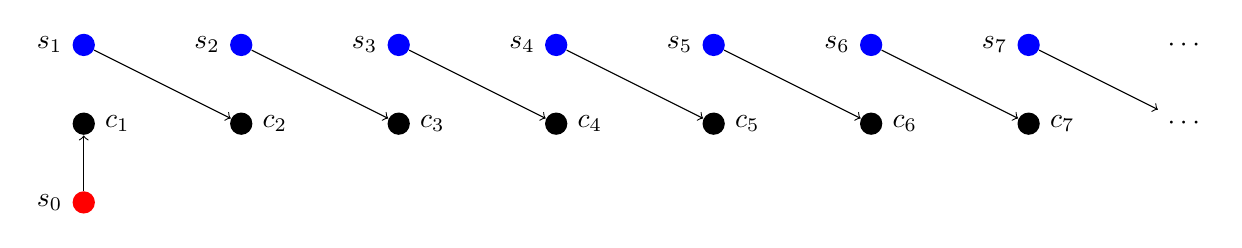
\begin{tikzpicture}
    \node[circle, fill=blue, inner sep=0.1cm, label=left:$s_1$] (s1) at (0, 1) {};
    \node[circle, fill=blue, inner sep=0.1cm, label=left:$s_2$] (s2) at (2, 1) {};
    \node[circle, fill=blue, inner sep=0.1cm, label=left:$s_3$] (s3) at (4, 1) {};
    \node[circle, fill=blue, inner sep=0.1cm, label=left:$s_4$] (s4) at (6, 1) {};
    \node[circle, fill=blue, inner sep=0.1cm, label=left:$s_5$] (s5) at (8, 1) {};
    \node[circle, fill=blue, inner sep=0.1cm, label=left:$s_6$] (s6) at (10, 1) {};
    \node[circle, fill=blue, inner sep=0.1cm, label=left:$s_7$] (s7) at (12, 1) {};
    \node[] (srest) at (14, 1) {$\cdots$};

    \node[circle, fill=black, inner sep=0.1cm, label=right:$c_1$] (c1) at (0, 0) {};
    \node[circle, fill=black, inner sep=0.1cm, label=right:$c_2$] (c2) at (2, 0) {};
    \node[circle, fill=black, inner sep=0.1cm, label=right:$c_3$] (c3) at (4, 0) {};
    \node[circle, fill=black, inner sep=0.1cm, label=right:$c_4$] (c4) at (6, 0) {};
    \node[circle, fill=black, inner sep=0.1cm, label=right:$c_5$] (c5) at (8, 0) {};
    \node[circle, fill=black, inner sep=0.1cm, label=right:$c_6$] (c6) at (10, 0) {};
    \node[circle, fill=black, inner sep=0.1cm, label=right:$c_7$] (c7) at (12, 0) {};
    \node[] (crest) at (14, 0) {$\cdots$};

    \node[circle, fill=red, inner sep=0.1cm, label=left:$s_0$] (s1n) at (0, -1) {};

    \draw[->] (s1) -- (c2);
    \draw[->] (s2) -- (c3);
    \draw[->] (s3) -- (c4);
    \draw[->] (s4) -- (c5);
    \draw[->] (s5) -- (c6);
    \draw[->] (s6) -- (c7);
    \draw[->] (s7) -- (crest);

    \draw[->] (s1n) -- (c1);
\end{tikzpicture}

Now every student is assigned to a chair, and every chair has a student. \reed{More explanation is probably need: clarify this is a good and complete assignment}
So then we \textbf{still} have as many chairs as students!
So adding one new student poses no issues: in fact, this also means that we can add two, three, four, etc. students.
How?
Just move everyone over one seat, then over again, etc.
\reed{This previous sentence should probably be an exercise}?
We could also say ``move everyone over two/three/four seats'', but then we have to define the assignment again; if we say move over one seat, then move over one more, we've achieved the same thing, but there's no need to prove that this works because we already have.
\reed{This previous sentence is only sort of true: we basically proved we can add one thing to natural numbers, but not that we can do it again...}

\paragraph{Adding Infinitely Many Students}
Intuitively, perhaps it makes sense that we can add any finite number of students to our class, because our class is so big that a finite addition basically makes no difference in the number of students.
But what if we want to add \textbf{infinitely more} students? For example, suppose we want to double the size of our class.
Specically, for every student $s_i$, we add a second student $s_{i}'$, but we don't add any more chairs.
Do we still have enough chairs for everyone?

At first glance, you might, quite reasonably, think there is no way that we could possibly have enough chairs for twice as many people.
We can't use our old strategy of just moving people over one at a time until we have enough seats, because we have to move over infinitely many times: we'll never finish!
It's very important that we be able to write down a complete description of our assignment; otherwise, how could anyone read it to tell what seat they should be in?
I don't mean that we have to list out the whole assignment, only that we have some finite way to describe the assignment; just enough to answer the question ``where should I sit?''
For example, if student 10, $s_{10}$ asks where they should sit, we can easily look at the (previous) assignment we gave, and say ``chair $c_{11}$.''
So if we can't use our old strategy, can we do it any other way, or is it impossible?

By impossible, I don't mean \textbf{really hard}, or ``I can't think of how to do it'', I mean, actually, provably, impossible.
For example, I can prove that you can't have a good assignment if you have $2$ students and only $1$ chair, or if you have infinitely many students, and finitely many chairs. \reed{Should we actually write out these proofs}

In fact, it is possible to assign each student in this new, larger class, to a chair; specfically, I claim there is a good, complete assignment.
Instead of telling everyone to move over one seat, we tell the first student to move over one chair, the second student to move over three, the third student to move over five, and so on.
Then the first new student sits in the first chair, the second new student sits in the third chair, the third new student sits in the fifth chair, and so on.
The diagram below shows this assignment:

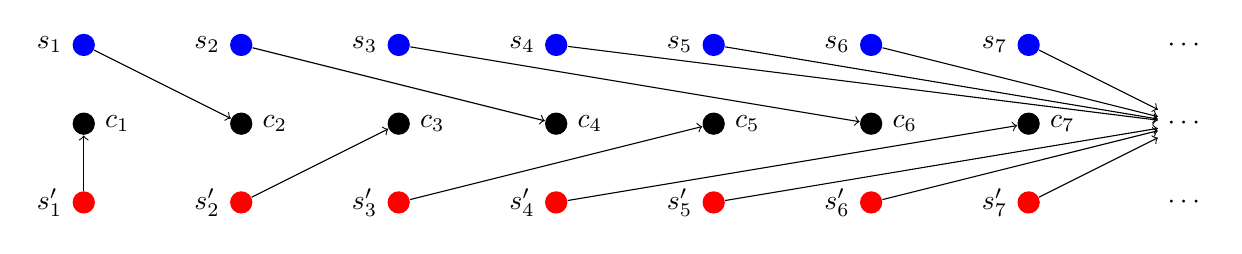
\begin{tikzpicture}
    \node[circle, fill=blue, inner sep=0.1cm, label=left:$s_1$] (s1) at (0, 1) {};
    \node[circle, fill=blue, inner sep=0.1cm, label=left:$s_2$] (s2) at (2, 1) {};
    \node[circle, fill=blue, inner sep=0.1cm, label=left:$s_3$] (s3) at (4, 1) {};
    \node[circle, fill=blue, inner sep=0.1cm, label=left:$s_4$] (s4) at (6, 1) {};
    \node[circle, fill=blue, inner sep=0.1cm, label=left:$s_5$] (s5) at (8, 1) {};
    \node[circle, fill=blue, inner sep=0.1cm, label=left:$s_6$] (s6) at (10, 1) {};
    \node[circle, fill=blue, inner sep=0.1cm, label=left:$s_7$] (s7) at (12, 1) {};
    \node[] (srest) at (14, 1) {$\cdots$};

    \node[circle, fill=black, inner sep=0.1cm, label=right:$c_1$] (c1) at (0, 0) {};
    \node[circle, fill=black, inner sep=0.1cm, label=right:$c_2$] (c2) at (2, 0) {};
    \node[circle, fill=black, inner sep=0.1cm, label=right:$c_3$] (c3) at (4, 0) {};
    \node[circle, fill=black, inner sep=0.1cm, label=right:$c_4$] (c4) at (6, 0) {};
    \node[circle, fill=black, inner sep=0.1cm, label=right:$c_5$] (c5) at (8, 0) {};
    \node[circle, fill=black, inner sep=0.1cm, label=right:$c_6$] (c6) at (10, 0) {};
    \node[circle, fill=black, inner sep=0.1cm, label=right:$c_7$] (c7) at (12, 0) {};
    \node[] (crest) at (14, 0) {$\cdots$};

    \node[circle, fill=red, inner sep=0.1cm, label=left:$s_1'$] (s1n) at (0, -1) {};
    \node[circle, fill=red, inner sep=0.1cm, label=left:$s_2'$] (s2n) at (2, -1) {};
    \node[circle, fill=red, inner sep=0.1cm, label=left:$s_3'$] (s3n) at (4, -1) {};
    \node[circle, fill=red, inner sep=0.1cm, label=left:$s_4'$] (s4n) at (6, -1) {};
    \node[circle, fill=red, inner sep=0.1cm, label=left:$s_5'$] (s5n) at (8, -1) {};
    \node[circle, fill=red, inner sep=0.1cm, label=left:$s_6'$] (s6n) at (10, -1) {};
    \node[circle, fill=red, inner sep=0.1cm, label=left:$s_7'$] (s7n) at (12, -1) {};
    \node[] (snrest) at (14, -1) {$\cdots$};

    \draw[->] (s1) -- (c2);
    \draw[->] (s2) -- (c4);
    \draw[->] (s3) -- (c6);
    \draw[->] (s4) -- (crest);
    \draw[->] (s5) -- (crest);
    \draw[->] (s6) -- (crest);
    \draw[->] (s7) -- (crest);

    \draw[->] (s1n) -- (c1);
    \draw[->] (s2n) -- (c3);
    \draw[->] (s3n) -- (c5);
    \draw[->] (s4n) -- (c7);
    \draw[->] (s5n) -- (crest);
    \draw[->] (s6n) -- (crest);
    \draw[->] (s7n) -- (crest);
\end{tikzpicture}

We can write this assignment as follows: assign student $s_i$ to chair $c_{2i+1}$, and student $s_i'$ to chair $c_{2i}$.
Hopefully it is clear from the diagram that each chair will only get one student, and that we will not ``run out'' of chairs to assign students to.
Furthermore, we won't ``miss'' any chairs: every chair gets a student.

So, perhaps surprisingly, there are as many students in our new, doubled class, as in our original class.
Remember, we agreed that if we have a good, complete assignment between a group of students and a group of chairs, then we have the same amount of students and chairs.
We have a good, complete assignment in our original class, and we have a good, complete assignment in our new, doubled class.
So if we have the same amount of students in the original class as chairs, and we have the same amount of students in the new class as we have chairs, then the amount of students in the original class must be the same as the amount of students in the new class.
To write this more concisely, denote the original class of students by $S$, the new class as $S'$, and the chairs by $C$.
Then what I'm saying is: because $\samenumber{S}{C}$ and $\samenumber{S'}{C}$, we can conclude that $\samenumber{S}{S'}$.

If you accept the above \reed{What to do if they don't?}, then we've discovered something somewhat strange.
Let's see how many students we can add to this class.
Essentially, what we did in the previous example is give each student a buddy, so there is a pairing of students, i.e., $s_i$ is ``paired with'' $s_i'$.
What if we gave each student $s_i$ two ``buddies'', $s_i'$ and $s_i''$?
Then we could do the assignment trick above once with $s_i$ and $s_i'$, then again with the new student paired with $c_i$ and $s_i''$ \reed{Clarify this sentence}.
As you can see, we can give each student in the original class any finite number of ``buddies'' (let's call this a group), and we can still find seats for everyone.
We just seat each group together, then move the following groups down by a corresponding amount.

So we can add a ``lot'' of students.
What if give each student infinitely many ``buddies''?
Specifically, for each student $s_i$, there are students $s_{i,1}$, $s_{i,2}$, $s_{i,3}$, and so on for every \reed{positive integer} $j$, there is a student $s_{i,j}$.
Surely that would be too many students?
We definitely can't use our old strategy of seating each group together, because then after the first ``group'', the second group would have to be infinitely far over!
So we're going to have to intersperse the students among each other.
\reed{Have them think about it?}

Again, perhaps very suprisingly, we still have enough chairs!
Consider the following picture, where each row represents one ``group'':

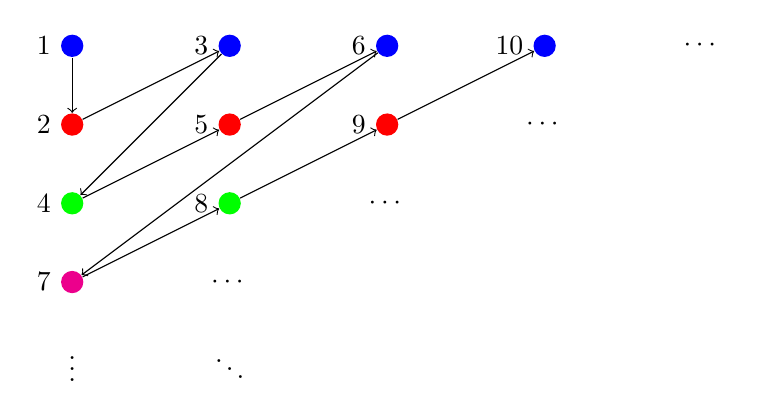
\begin{tikzpicture}
    \node[circle, fill=blue, inner sep=0.1cm, label=left:$1$] (s11) at (0, -1) {};
    \node[circle, fill=blue, inner sep=0.1cm, label=left:$3$] (s21) at (2, -1) {};
    \node[circle, fill=blue, inner sep=0.1cm, label=left:$6$] (s31) at (4, -1) {};
    \node[circle, fill=blue, inner sep=0.1cm, label=left:$10$] (s41) at (6, -1) {};
    \node[] (srest) at (8, -1) {$\cdots$};

    \node[circle, fill=red, inner sep=0.1cm, label=left:$2$] (s12) at (0, -2) {};
    \node[circle, fill=red, inner sep=0.1cm, label=left:$5$] (s22) at (2, -2) {};
    \node[circle, fill=red, inner sep=0.1cm, label=left:$9$] (s32) at (4, -2) {};
    \node[] (srest) at (6, -2) {$\cdots$};

    \node[circle, fill=green, inner sep=0.1cm, label=left:$4$] (s13) at (0, -3) {};
    \node[circle, fill=green, inner sep=0.1cm, label=left:$8$] (s23) at (2, -3) {};
    \node[] (srest) at (4, -3) {$\cdots$};

    \node[circle, fill=magenta, inner sep=0.1cm, label=left:$7$] (s14) at (0, -4) {};
    \node[] (srest) at (2, -4) {$\cdots$};

    \node[] (s1) at (0, -5) {$\vdots$};
    \node[] (s2) at (2, -5) {$\ddots$};

    \draw[->] (s11) edge (s12)
              (s12) edge (s21)
              (s21) edge (s13)
              (s13) edge (s22)
              (s22) edge (s31)
              (s31) edge (s14)
              (s14) edge (s23)
              (s23) edge (s32)
              (s32) edge (s41);
\end{tikzpicture}

We can assign the students by starting at the top left corner, and moving along the grid diagonally, as shown below.
That is, $s_{1,1}$ is assigned to seat $1$, $s_{1,2}$ is assigned to seat $2$, $s_{2,1}$ is assigned to seat $3$, and so on.
Again, we can see that if we go far enough, we can get every student.

\paragraph{Is it possible to have too many students?}

\paragraph{What are the properties of ``same amount''?}
\reed{Maybe an interesting digression, but perhaps they are not yet convinced that this is interesting enough to talk about formal properties}
This brings up a couple of questions.
My logic in the previous paragraph was as follows:

\begin{enumerate}
    \item Suppose I have three groups of objects, $A$, $B$, and $C$.
    \item I know that $\samenumber{A}{B}$ and $\samenumber{C}{B}$.
    \item So then $\samenumber{A}{C}$.
\end{enumerate}

This brings up a new question: if I have three groups of objects, $A$, $B$, and $C$, and I know that $\samenumber{A}{B}$ and $\samenumber{C}{B}$, can I say that $\samenumber{A}{C}$?

\section{The Kinds of Infinity}

In the previous section, we established that there are multiple kinds, or sizes, of infinity.
Or, at least, there are two: the things that are the same size as the positive integers, and the things that are as many as groups of positive integers.

\subsection{Some New Language}

Our language, while quite versatile, is not quite ideal for the topic at hand.
That previous sentence is probably very difficult to read, and is even more difficult to talk about with other people.
In fact, many of the previous sentences are, despite the author's best effort, difficult to parse.

To fix this problem, we're going to introduce some new words to make talking about groups and infinities a bit easier.

First, we're going to introduce so new terms for things we've been saying; in particular, we want to replace some common English terms with their technical versions, because using plain English terms can be misleading if we don't mean them in a colloquial sense.
Instead of ``group'', we'll use \emph{set} or \emph{collection}.
The things inside a set or collection are called \emph{elements}.
Note that order in a set doesn't matter, the set $\curlys{1,2}$ is the same as the set $\curlys{2,1}$; we only care what's in the set.
Instead of ``amount'', we will use \emph{cardinality}.
Then, instead of saying ``we have the same amount of students in the original class as there are chairs'', we'll say ``the collection of students in the new class has same cardinality as the set of chairs.''
This isn't shorter, but it's more precise: any mathematically trained person will know what we mean; if we use ``group'' and ``amount'', it's too vague to be sure what we're really talking about without going into more detail.
Instead of saying ``the set $A$ has the same cardinality as positive integers'', we'll say ``$A$ is \emph{countable}'', or ``there are \emph{countably many} elements of $A$''.
If some set is too big to have a good, complete assignment with a countable set, we'll say it is \emph{uncountable}.
Finally, instead of ``groups of things in a set $X$'' we'll say ``\emph{subsets} of $X$''; so then we can say ``the set of subsets of positive integers is uncountable.''
\reed{Is this too many new definitions to just throw at them?}
\reed{Should definitions be more rigorous?}

For some examples, $\curlys{1,2,3}$ is a group of things in the bigger group $\curlys{1,2,3,4,5}$, so $\curlys{1,2,3}$ is a \textbf{subset} of $\curlys{1,2,3,4,5}$.
Similarly, $\curlys{1}$ is a subset of $\curlys{1,2,3,4,5}$.
Finally, note that we consider the ``empty group'' or \emph{empty set}, $\emptyset := \curlys{}$, which has no elements to be a subset of \textbf{every} set.
\reed{How to build familiarity with the empty set and sets in general, but maintaining the flow?}
\reed{Is this even important right now?}

\subsection{How many sizes of infinity?}

As briefly discussed earlier, we've so far found two different kinds of infinity: countable and uncountable.
Is that all there is: specfically, if a set is uncountable, it is the same size as every other uncountable set?
\reed{I have literally no intuition for guessing what people will think about this...}

The answer is no, and we'll need one more term to talk about it: the \emph{powerset} of a set is the set of all subsets of that set.
So the powerset of $\curlys{1,2,3}$ is $\curlys{\emptyset, \curlys{1}, \curlys{2}, \curlys{3}, \curlys{1,2}, \curlys{1,3}, \curlys{2,3}, \curlys{1,2,3}}$.
By convention, for a set $A$, we consider both $\emptyset$ and $A$ to be subsets of $A$.
\reed{Should probably explain this convention...}
We write ``the powerset of a set $A$'' as $\powerset{A}$.
Then we can rephrase the earlier sentence about the powerset of $\curlys{1,2,3}$ as:

\[
    \powerset{\curlys{1,2,3}} = \curlys{\emptyset, \curlys{1}, \curlys{2}, \curlys{3}, \curlys{1,2}, \curlys{1,3}, \curlys{2,3}, \curlys{1,2,3}}
\]

Then we have the following theorem:

\begin{theorem}
    For any set $A$, the cardinality of the powerset of $A$, $\powerset{A}$, is greater than the cardinality of $A$; that is:

    \[
        \abs{\powerset{A}} > \abs{A}
    \]
\end{theorem}

\begin{proof}

\end{proof}

\subsection{Different Kinds of Numbers}

We've discussed and used a variety of different kinds of numbers throughout this book.
First, we talked about \reed{positive integers}: $1$, $2$, $3$, $4$, $5$, etc.

But there are, of course, other kinds of numbers: what about $0$, $-10$, $\frac{1}{2}$, or the famous $\pi$?
Each of these numbers is a representative of a different kind of numbers.
Each kind of numbers forms a set of numbers.

We call the numbers $0$, $1$, $2$, $3$, $4$, $5$, and so on the \emph{natural numbers}, because they are ``natural'' in the sense that they are obviously useful for counting.
We denote the set of all natural numbers by $\nat$, which is just a fancy way to write an $N$.

The numbers like $-10$, $-5$, $2$, or $129$ are called \emph{integers}, coming from the Latin \emph{integer}, meaning ``whole''.
We can clearly see that every natural is itself an integer, but we also include the natural numbers.
\reed{Is this actually that obvious...I think so?}
We write the set of integers as $\integers$, because the German word for ``numbers'' is \emph{Zahlen}.

Next, we have numbers like $\frac{5}{2}$, $-\frac{11}{2}$, $\frac{129}{1819}$, and so on.
These numbers are called \emph{rational numbers}, because they are ``ratios'' of integers (where the bottom number is not $0$).
We write the set rational numbers as $\rational$ for ``quotient''.

\subsection{How many of each kind of number are there?}


\section{Ordinals}

The most natural way to represent the size of a finite set is by saying how many elements it has; this number is always a natural number.
Ideally, we'd also have some ``numbers'' that let us discuss the sizes of infinite sets.

But have you ever wondered what numbers are?
As in, \textbf{what is zero?}
\textbf{What is one?}
Or why does $1 + 1 = 2$?
And why does $4 + 2 = 4 + 2$?
And why does that work for all numbers?
Does it work for all numbers?

Well, I won't answer all those questions necessarily, but I will answer some of them.

\subsection{Defining the natural numbers}

Hopefully you aren't tremendously disappointed, but the objective of math is rarely to answer the question ``What \textbf{really} is $X$?''
Instead, we generally ask: ``What are the essential properties of $X$?''
We can also choose to define representations of objects, and if these representations conform to all the properties, then we may just end up saying that they ``really'' \textbf{are} the object, if it becomes convenient.
This, for us, is one of those cases.

Let's start defining some natural numbers.
What are the most basic objects we can talk about, without needing to rely on any other definitions?
We can't say something like ``$3$ means $3$ apples'' or something, because then we need to define apples.
We could just say $0$ is some object with some properties (perhaps that $0 + x = 0$), but we already know of some object that, in many ways, acts just like $0$ does: the empty set.
If I take any set, and I take all the elements in that set and I add the elements of the empty set, then I have the same elements as I did before.
So this property is a lot like the fact that we all know and love, that $0 + x = 0$.
So we'll define $0$ to be $\emptyset$; we write $0 := \emptyset$ to mean that $0 = \emptyset$, and that this is true \emph{by definition}.

This is a fundamental principle of this business of precisely defining objects: there are some properties we want to preserve, and we looks for simpler objects that we already know that have these same properties.
Along the way, we may need to define new notions \reed{should I use a word other than ``notions'' here...} and objects; this is more generally part of the process of mathematical modeling.

We've defined one natural number, the smallest one, which is a good start, but what about the rest of the natural numbers?
Let's consider one other property of the natural numbers: we can get any natural number by just adding $1$ to $0$ a bunch of times.
For example, $4 = 0 + 1 + 1 + 1 + 1$, and $5 = 0 + 1 + 1 + 1 + 1 + 1$.
You can see how this pattern will continue; so I won't write them all out.
So really, we don't actually need to write every single number out, we just need to define what it means to ``add $1$'' to a natural number, and we can get all the rest of the natural numbers.
And to do this, we'll consider one last property of natural numbers: specifically, how do we order natural numbers?
That is, we know that $0 < 1 < 2$, and $0 < 1 < 2 < 3$, and so on.
So the set of natural numbers less than $3$ is $\curlys{0,1,2}$, the set of natural numbers less than $2$ is $\curlys{0,1}$, the set of natural numbers less than $1$ is just $\curlys{0}$, and finally the set of natural numbers less than $0$ is $\emptyset$, because there are no natural numbers less than $0$.
But wait!
We defined $0$ to be $\emptyset$; what if we just defined $1$ to be $\curlys{0}$, and $2$ to be $\curlys{0,1}$, and so on.
That is, each natural number is the set of numbers that are less than it, and ``adding one'' means including the currently number in this collection.

To write the previous sentence in symbols, let's define $n + 1 := n \cup \curlys{n}$.
What does $\cup$ mean?
$\cup$ is used to write the \emph{union} of two sets.
Below is a precise definition of what that means:

\begin{definition}
    For any sets $A$ and $B$, the set $A \cup B$ is the set of all elements that are in either $A$ or $B$, or both.
    That is, $x \in A \cup B$ if and only if $x \in A$ or $x \in B$.
\end{definition}

For example, $\curlys{1,2} \cup \curlys{3,4} = \curlys{1,2,3,4}$, and $\curlys{a,b,c} \cup \curlys{a,d,f} = \curlys{a,b,c,d,f}$.
Note that sets never contain ``repeats'': we can specify a set by just saying what's inside it, without specifying \textbf{how many} of that thing are in the set.

Let's verify that this definition actually works.
We already agreed that $0 = \emptyset$, so then:
\begin{align*}
    0 + 1 &= \emptyset \cup \curlys{\emptyset} = \curlys{\emptyset} = \curlys{0} \\
    1 + 1 &= 1 \cup \curlys{1} = \curlys{\emptyset} \cup \curlys{\curlys{\emptyset}} = \curlys{\emptyset, \curlys{\emptyset}} = \curlys{0, 1} \\
    2 + 1 &= 2 \cup \curlys{2} = \curlys{\emptyset, \curlys{\emptyset}} \cup \curlys{\curlys{\emptyset, \curlys{\emptyset}}} = \curlys{\emptyset, \curlys{\emptyset}, \curlys{\emptyset, \curlys{\emptyset}}} = \curlys{0, 1, 2} \\
    &\vdots
\end{align*}

This definition has the nice property that if $n \in m$, then $n < m$: for example $0 \in 1$, because $0 = \emptyset$ and $1 = \curlys{\emptyset}$.
In fact, because we're trying to define the natural numbers ``from scratch'', this will work for us as a \textbf{definition} of what it means for one natural number to be less than another.

This is the beginning of a definition of the natural numbers, but it is important to note that this isn't the \textbf{only} definition of the natural numbers; there are many, (essentially) equivalent definitions which are appropriate for different situations.

\subsection{Defining arithmetic on natural numbers}

Let's step back for a moment, and take stock of what we've done:

\begin{enumerate}
    \item Defined $0 := \emptyset$
    \item Defined, for any natural number $n$, $n + 1$
    \item Defined what is means for two natural numbers $n$ and $m$ to be less than each other, specifically $n \in m$ means that $n < m$.
\end{enumerate}

What other things might we like to do with natural numbers?
Naturally, we might like to add them, multiply them, and so on.
Let's define addition first, again, being careful to do so only in terms of things we have already defined.
We'll define addition of two natural numbers, $n$ and $m$, as follows:
\begin{align*}
    n + 0 &:= n \\
    n + (m + 1) &:= (n + m) + 1 \\
\end{align*}

Above, we've defined what it means to do $n + 1$, and we just declare that $n + 0 := n$.
Let's do an example of addition:
\[
    1 + 2 = 1 + (1 + 1) = (1 + 1) + 1 = 2 + 1 = 3
\]

Basically, our objective is to ``convert'' the operation of doing $n + m$ into just doing $n + 1 + 1 + \cdots + 1$, because we know how to add $1$ to a natural number.
If you've ever heard ``addition just counting'' \reed{I think there's some more common way that this usually gets phrased}, well, that's true for natural numbers, and that's how we choose to define addition.
And if you've ever heard ``multiplication is just repeated addition'', you'll know how we're going to define multiplication.

\begin{align*}
    n \cdot 0 &:= 0 \\
    n \cdot (m + 1) &:= n + n \cdot m
\end{align*}

\reed{show that we can take max and min by using unions and intersections}

\subsection{Some properties of natural numbers}

Let's step back again, now that we've defined a whole bunch of operations on natural numbers, and look at some properties of natural numbers.
Let's write out a few natural numbers so we can see some patterns:

\begin{itemize}
    \item[] $0 = \emptyset$
    \item[] $5 = \curlys{0,1,2,3,4}$
    \item[] $6 = \curlys{0,1,2,3,4,5}$
    \item[] $10 = \curlys{0,1,2,3,4,5,6,7,8,9}$
\end{itemize}

Specifically, there's a couple important properties here: which we can see what we look at $5$ and $6$.
In fact, maybe it's so obvious that it doesn't even seem to warrant mention, but let's not that not only do we have $5 \in 6$, we also have $5 \subseteq 6$!
Said another way, this is somewhere less surprising: we know that $2 < 5$, and $5 < 6$, so this is just saying that $2 < 6$.
Put yet another way, we know $2 \in 5$, and $5 \in 6$, and $5 \subseteq 6$, so $2 \in 6$.

If you're familiar with the transitive property in general, that if $x < y$ and $y < z$, then $x < z$, you'll recognize this as being something similar.
In fact, let's make preicse what we've been saying, and come up with a general definition of ``transitive'' as it relates to sets:

\begin{definition}
    A set $X$ is called \emph{transitive} if for any $Y \in X$, $Y \subseteq X$.
\end{definition}

Let's now discuss perhaps the most important property of the natural numbers, called \emph{well-ordering}, which says that any subset of the natraul numbers has a smallest element.
To see why this statement is important, or indeed, why this statement really has any meaning at all, let's consider some sets for which it is not true.

\begin{example}
    The set of integers, $\integers$, is not well-ordered, because there is no smallest integer.
\end{example}

In retrospect, this maybe seems obvious, and is probably not what you were thinking of.
Perhaps you were picturing a \emph{bounded} set, such as the integers greater than $-10$ and less than $10$ (or even just greater than $-10$), which certainly does have a least element.
However, if we consider the real numbers, taking again our favorite example---the real numbers between $0$ and $1$ (not including $0$)---we can again see that there even though this set is bounded, both above and below \reed{Should we define these terms, or avoid them, or just not worry about it?}, there is no least element, because we can always halve a number and get a smaller number that's still in the set \reed{is this 100\% obvious? does it merit more explanation}
Now that you're perhaps convinced why well-ordering is a somewhat special property \reed{should we do more on this topic?}, let's give it a proper definition.

\begin{definition}
    A set $A$ is well-ordered if every nonempty subset $B$ of $A$ has a least element.
\end{definition}

Not only are the natural numbers well-ordered, but every natural number is itself well-ordered: any nonempty subset of a natural number $n$ is a subset of the natural numbers.
\reed{elaborate?}

\reed{We should probably talk a little bit more about something stuff here, or give more examples}

\subsection{Ordinals}

Let's expand our definition of natural numbers a little bit, because we want to talk more generally about the sizes of sets, and natural numbers only let us discuss the sizes of finite sets.
That is, we need to start defining infinite numbers.
Despite what you may have heard, it is absolutely possible to talk coherently about infinity, and even infinitely large numbers: in fact, we've already discussed the topic of infinity quite frequently, in discussing the various sizes of infinite and schemes for comparing different infinite sets.

First, let's look at what we did before, defining a natural number to be the set of all natural numbers less than it, and let's look at other things we already know about; specifically, the set of natural numbers, $\nat$, itself.
Firstly, every natural number is a set of natural numbers: that is, for every $n \in \nat$, we also have $n \subseteq \nat$: so $\nat$ is transitive!
Additionally, we already know that $\nat$ is well-ordered. \reed{Should we like, prove this at some point, or?}

So $\nat$ has two of the important properties of natural numbers.
That is, for our purposes, it's somewhat natural number-like.
However, it'd be quite misleading to call it a \textbf{natural number}, so we'll invent a new term for this sort of number: they're called \emph{ordinals}, and they're traditionally denoted by Greek letters, starting with $\alpha$, $\beta$, and $\gamma$, so we'll follow that tradition.
\reed{At some point should we describe why following conventions like this is important? That's probably an important thing, but not sure if it needs to be made explicit. in general, we should tlak about notation and stuff}

\begin{definition}
    A set $\alpha$ is called an \emph{ordinal} if it is transitive and well-ordered by $\in$.
\end{definition}

As we have already seen, all natural numbers are ordinals.
However, $\nat$ is an ordinal, and not a natural number, so not \textbf{all} ordinals are natural numbers.
Additionally, because every natural number is an element of $\nat$, $\nat$ is an ordinal bigger than any other natural number.
That is, $\nat$ is a sort of infinite number: when we want to emphasize that $\nat$ is a infinite ordinal, we'll usually write $\omega_0$ instead of $\nat$, but they're the same thing.

This also brings up to one more incredibly important realization.
For all the natural numbers, we could get to any other natural number just ``adding one'', which we'll call the \emph{successor} from now.
However, this is obviously not the case for $\omega_0$: if we have some natural number $n$, we can't add $1$ any finite number of times to get $\omega_0$.
Put another way, for any natural numbers $n$ and $m$, $n + m < \omega_0$.
So then $\omega_0$ is not the successor of \textbf{any} ordinal!

This leads us to the realization that there are multiple, natural, classes of ordinals: successor ordinals, like the natural numbers, and limit ordinals, like $\omega_0$.
In fact, there's a third kind: $0$.
$0$ isn't the successor of any ordinal, because it's the smallest ordinal, but it's also not really a limit in the same way that $\omega_0$ is, so it get's it's own class.
Let's give some more precise definitions for the various types of ordinals:

\begin{definition}
    An ordinal $\alpha$ is a \emph{successor} ordinal if there is some ordinal $\beta$ so that $\alpha = \beta + 1$.
\end{definition}

\begin{definition}
    An ordinal $\alpha$ is call a \emph{limit} ordinal if for every $\beta < \alpha$, $\beta + < \alpha$.
\end{definition}

So we know that every natural number is an ordinal, and the set of natural numbers is an ordinal...what other ordinals are there?
Well, our previous strategy for building more ordinals was to just take successors.
So why not try that again?
What is $\omega_0 + 1$?

Well, by definition, it's $\omega_0 \cup \curlys{\omega}$, which certainly is \textbf{something}...but is it an ordinal?
The question I'm asking might be phrased more mathematically as: ``is the successor of an ordinal still an ordinal?''
The answer is ``yes'', and the reason will be laid out in the following proof.
Note that we call this result a ``lemma'' rather than a ``thereom'' because it is not a huge, wide reaching fact, but it is a small fact that is often very useful. \reed{Should we clarify?}
\reed{At some point, we should move over to more proofs and stuff, but when should that be?}

\begin{lemma}
    For any ordinal $\alpha$, it's successor, $\alpha + 1$, is also an ordinal.
    \reed{this is a rather formal/abstract thing, maybe we don't need to worry about proving it right now}
\end{lemma}
\begin{proof}
    We need to show both that $\alpha + 1$ is transitive and that it is well-ordered by $\in$, meaning that any nonempty subset of $\alpha$ has a least element.

    Let's first show that it is transitive.
    To do so, we need to show that any element of $\alpha + 1$ is a subset of $\alpha + 1$, so for any $\beta \in \alpha + 1$, $\beta \subseteq \alpha + 1$.

    Suppose that we have some element $\beta \in \alpha + 1$.
    Then because $\alpha + 1 = \alpha \cup \curlys{\alpha}$, either $\beta \in \alpha$ or $\beta \in \curlys{\alpha}$, by definition of the union.
    Let's consider these two cases separately.
    If $\beta \in \alpha$, then we know that $\beta \subseteq \alpha$, because $\alpha$ is an ordinal and therefore $\alpha$ is transitive.
    Also, we know that $\alpha \subseteq \alpha + 1$, because $\alpha + 1 = \alpha \cup \curlys{\alpha}$; and that's all we wanted to show for now.
    \reed{Should we explain/prove that $A \subseteq A \cup B$?}
    Now let's suppose that $\beta \in \curlys{\alpha}$; but that means that $\beta = \alpha$, because $\curlys{\alpha}$ only has one element.
    But as we just discussed, $\alpha \subseteq \alpha + 1$, so $\beta \subseteq \alpha + 1$, just like we wanted.

    Now let's show that $\alpha + 1$ is well-ordered by $\in$.
    That means that we need to show that for any nonempty subset $Y \subseteq \alpha + 1$, there is some $\in$-least element of $Y$.
    \reed{Explain $\in$-least?}

    So let's suppose we have some nonempty subset $Y \subseteq \alpha + 1$, and again we'll consider two cases, either $\alpha \in Y$ or $\alpha \not\in Y$.
    Let's suppose that $\alpha \in Y$.
    Now let's consider two more cases: either $Y = \curlys{\alpha}$, or there is some other element of $Y$, which we'll call $\beta$.
    If $Y = \curlys{\alpha}$, then $\alpha$ is the $\in$-least element of $Y$ because it's the only element of $Y$.
    Otherwise, there must be some other element $\beta \in Y$, that means that $\alpha$ and $\beta$ are different.
    In this case, $\beta < \alpha$, because $\alpha$ is the biggest element in $\alpha + 1$ \reed{Does this need more explanation?}.
    So then the least element of $Y$ must be less than $\alpha$, so the least element of $Y$ must be the same as the least element of $Y$ without $\alpha$.
    However, $Y$ without $\alpha$ is a subset of $\alpha$ \reed{explain?}, so because $\alpha$ is well-ordered by $\in$, there is some $\in$-least element of $Y$.
    Finally, let's consider the case that $\alpha \not\in Y$.
    In this case, we know that $Y \subseteq \alpha$, so again using the fact that $\alpha$ is well-ordered by $\in$, as it is an ordinal, we can use that to get our least element of $Y$.

    This completes, the proof: the successor of every ordinal is also an ordinal!
\end{proof}

This proof means there are \textbf{lots} of ordinals!
In fact, we have ordinals $\omega_0$, $\omega_0 + 1$, $\omega_0 + 2$, $\omega_0 + 3$, and so on.
But how many ordinals are there?
Let's consider the following set: $\omega_0 \cup \curlys{\omega_0, \omega_0 + 1, \omega_0 + 2, \ldots}$, that is, the set of natural numbers unioned with $\omega_0 + n$ for every natural number $n$.
Is this set an ordinal?
It is certainly transitive, because anything in it is either a natural number or $\omega_0 + n$ for some natural number; the natural numbers are all subsets of $\omega_0$, and $\omega_0 + n$ is a subset of $\omega_0 + (n + 1)$.
\reed{Is this proof too quick?}
But is it well-ordered by $\in$?
Indeed, it is: suppose we have some nonempty subset $A$ of this set; because it's nonempty there must be \textbf{some} $\alpha \in A$.
If $\alpha = \emptyset$, then it is the least element, because nothing is less than $0$ (in the natural numbers/ordinals).
However, if it is not, then let's consider the set $\alpha \cap A$: the set of all ordinals that are both in $A$ and $\alpha$.
Note that, because $\alpha$ is an ordinal, there is some least element $\beta \in \alpha \cap A$, and $\beta$ must also be the least element of $A$.
We can see that this last part is true because if there were some other $\gamma \in A$ that was smaller than $\beta$, then $\gamma \in \beta$, and so $\gamma \in \alpha$, so $\beta$ is not the smallest element of $\alpha$ after all.

In fact, this last fact we've proven is quite useful, so let's declare it as a lemma.

\begin{lemma}\label{lem:nonemptyOrdIsOrd}
    If $A$ is a nonempty set of ordinals, then $A$ has a least element.
\end{lemma}
\begin{proof}
    See above, and notice that our proof works for any nonempty set of ordinals, not just the subsets we were considering above.
\end{proof}

This also gives us another useful fact about how to create new ordinals:
\begin{lemma}\label{lem:transSetOfOrdIsOrd}
    If $A$ is a transitive set of ordinals, then $A$ is itself an ordinal.
\end{lemma}
\begin{proof}
    We only need to show that $A$ is well ordered by $\in$, because we already assumed that it is transitive.

    If $A = \emptyset$, then we know that $A$ is an ordinal already.
    If not, then there is some element in $A$, so it is a nonempty set of ordinals.
    If we have some nonempty subset of it, then we know by Lemma \ref{lem:nonemptyOrdIsOrd} that this nonempty subset has a least element.
\end{proof}

Let's talk about one more nice fact about ordinals.
\reed{more motivation}
\begin{lemma}\ref{lem:inOrdIsOrd}
    For an ordinal $\alpha$, any $\beta \in \alpha$ is also an ordinal.
\end{lemma}
\begin{proof}
    Let's take some $\beta \in \alpha$ for some ordinal $\alpha$.
    We want to show that $\beta$ is both transitive and well-ordered by $\in$.

    First, let's show that it is transitive, so if we take some $\gamma \in \beta$, then we want to show that $\gamma \subseteq \beta$.
    Because $\alpha$ is transitive, and $\beta \in \alpha$, we know that $\beta \subseteq \alpha$.
    We also know that $\gamma \in \beta$, so that gives us that $\gamma \in \alpha$ and also that $\gamma \subseteq \alpha$ by using the transitivity of $\alpha$ again.
    We want to know that $\gamma \subseteq \beta$, so let's take the standard approach of taking some $\delta \in \gamma$ and showing that $\delta \in \beta$.
    Note that all three of $\delta$, $\gamma$, and $\beta$ are in $\alpha$, and $\alpha$ is well-ordered by $\in$, so $\delta \in \gamma \in \beta$, which we know, gives us that $\delta \in \beta$.
    \reed{Should probably do more picture proofs or something}

    The last thing is to show that $\beta$ is well-ordered by $\in$, or that every nonempty subset of $\beta$ has a least element.
    However, if we have some nonempty subset $A$ of $\beta$, then $A$ is also a nonempty subset of $\alpha$ because $\alpha$ is a transitive set.
    So then because $\alpha$ is well-ordered by $\in$, there is some least element of $A$, and $\beta$ is also well-ordered by $\in$.
\end{proof}

\reed{Should we construct uncountable ordinals without AXiom of choice (a la Hartogs?) probalby unnecessary, doubt the intended audience is worried about the axiom of choice}
\reed{Here we should eventually define the set of all ordinals, then derive some wacky wacky shit and be like ``wait this isn't right...''}

Let's now consider the set of all ordinals, which we'll call $\bm{Ord}$, and see what kind of statement we can make about this set.
For example, maybe we want to ask how big it is?
Are there as many ordinals as there are real numbers?
What about the powerset of the real numbers, or the powerset of the powerset of the real numbers, and so on?
Certainly it's at least as big as the natural numbers, for several reasons.
For one, it contains the natural numbers; secondly, it is infinite, and we've already seen that every infinite set is at least as large as the natural numbers.

To answer this ``basic'' question, let's notice some facts about this set.
Firstly, every element of this set is an ordinal, so if we have some $\beta \in \bm{Ord}$, then $\beta$ is a ordinal.
This is nothing surprising, because that's literally how we defined the set.
However, notice that, as we just proved in Lemma \ref{lem:inOrdIsOrd}, every element of $\beta$ is also an ordinal.
So that means that every element of $\beta$ is also in $\bm{Ord}$, because that's how we defined $\bm{Ord}$, so then $\beta \subseteq \bm{Ord}$.
But wait: that means that $\bm{Ord}$ is a transitive set of ordinals, and by Lemma \ref{lem:transSetOfOrdIsOrd}, that means that $\bm{Ord}$ \textbf{is} an ordinal!
And that means that $\bm{Ord} \in \bm{Ord}$, so then $\bm{Ord}$ is a set that contains itself!

Is that possible?
On one hand, it seems very strange.
On the other hand, probably so did the fact that there are as many rational numbers as natural numbers.
So maybe our intuition doesn't line up here.
How can we prove that this really is impossible?
And if we can prove this, then that means we just proved a false statement, which definitely can't be done...but where did we go wrong?
At each step, it seems we've been extremely logical, at times, perhaps overly so.
In fact, we can see that this statement is a contradiction: by definition of an ordinal, every ordinal is well-ordered by $\in$.
That means that $\in$ is irreflexive, so $x \not\in x$ for any ordinal $x$.
Except we just showed that $\bm{Ord} \in \bm{Ord}$, and obviously a statement cannot both be true and false. \reed{presumably they will accept this as being ``obvious''}

So we just proved a false statement, using seemingly logical methods.
Does that mean that anything goes?
If we can prove one false statement, can't we prove them all? \reed{Maybe the principle of explosion is not obvious?}

Let's say we're trying to prove some statement $B$, and we know that $A$ is both true and false.
If $B \implies A$, then $\neg A \implies \neg B$, so $\neg B$ is true.
Otherwise, $B$ does not imply $A$, which means that $B$ is true and $A$ is not true.
But we know that $A$ is true, so then $B$ must not be true, so $B$ is false.
So then every statement is false... \reed{idk how convincing this is}

That seems a little hard to accept, so let's explore a more likely solution: we made a mistake in one of the prior proofs?
Which one was it?
\reed{Probably should have people consider this at some point}


\section{Sets}

So far we've only talked about sets in a very informal sense, and we've briefly discussed a couple operations.
For example, I've said that $\curlys{1,2,3}$ is a set of three numbers, and that if I have two sets $A$ and $B$, I might take their union $A \cup B$ which is the set containing all the elements in $A$ and all the elements in $B$.
For finite sets, this all seems pretty intuitive, and it seems unlikely that we can go wrong with anything that's vaguely described in this manner.

However, for infinite sets, we have to realize that our intuition is often wrong, or at least incomplete.


\section{Truth}

Some statements are true; others are false.
How do we \textbf{know}, for sure, what is true?
Can we know at all?

Well, some statements, at least, uncontroversial: for example, $1 = 1$.
In general, if I have anything, let's call it $x$, $x = x$ is definitely true.
So then the statement ``for any $x$, $x = x$ is true'' is, itself, a true statement.

Let's ask another very basic, uncontroversial question: are there things?
I think you will not protest when I say, ``yes, there are things.''
In fact, let's weaken this a little bit: ``yes, there is a thing.''
It's generally true that it's easier to show there is at least one thing than that there are multiple things; moreover, it often is unimportant how many things there are, if there is at least one thing.
For example, if there is a route from your house to the store, it doesn't really matter that there are multiple routes from your house to the store (even though this is almost certainly the case).

More generally, \emph{tautologies}, or statements that is always true: like ``a true statement is true'' and ``a false statement is false'' are true.
Less abstractly, it could be a statement like ``either I have class today or I don't have class today.''

Let's introduce some terminology to make the rest of this book less cumbersome.
We will introduce \emph{variables} for \emph{statements}.
So then, instead of saying ``a statement'' or ``the first statement'', I will say ``suppose A is a statement''.
We'll define exactly what statements are soon, but for now, you can think of it of being basically any sentence.

\paragraph{Basic statements}

Some of the most basic statements are the statements ``a true statement is true'' and ``a false statement is true'' (which it, itself, clearly false).
From now on, we'll refer to these as $\top$, or ``True'', and $\bot$, or ``False'', respectively.

These two form the basis of all statements we can make; but what other statements can we make?
Earlier we said that we can say that $x = x$ for any ``thing'' (to be defined later) $x$, so let's add that to the list of basic statements.

\paragraph{The Meaning of Words}

Let's talk about combining statements now in various ways that you're probably familiar with.
Below $A$ and $B$ are arbitrary statements.

Firstly, if I know that $A$ is true, then the statement ``$A$ is true'', is, itself true.
For example, the sentence ``$1 = 1$ is true'' is the same as saying ``$1=1$''.
Therefore, sometimes we will shorten things by just writing ``suppose $A$'' instead of ``suppose $A$ is true.''

If I know that $A$ is true and $B$ is true, then I know that ``$A$ and $B$'' is true.
For example, I know that ``$1 = 1$'' and ``$2 = 2$'' are true statements, so I always know that ``$1 = 1$ and $2 = 2$'' is a true statement.
This, like many of the examples in this chapter, are quite obvious: on the other hand, they're also quite useful.
Our objective is to build up the number of things that we know to be true, without a doubt, until we can answer interesting questions.
So we know that if we have two true statements $A$ and $B$, we can combine them into a new statemnet, ``$A$ and $B$'' that is also true.

But there are other ways to combine statements.
If I know that either $A$ is true, or $B$ is true, or perhaps both are true, then the statement ``$A$ or $B$'' is true.
We choose to say that if both are true, ``$A$ or $B$'' is true because it simplifies things: this is called an \emph{inclusive or}.
There's also the \emph{exclusive or}, which is perhaps more familiar, in which ``$A$ (exclusive) or $B$'' would be true if $A$ is true or $B$ is true, but not both.

It is quite cumbersome to write long sentences to describe obvious things, so we will state to write these facts in a more concise way.
For example, we will write our rule that if I know that $A$ is true and $B$ is true, then ``$A$ and $B$'' is true as follows:

\begin{mathpar}
    \inferrule{A \and B}{A \tand B}
\end{mathpar}

We read that as ``given `$A$' and `$B$', we can conclude `$A$ and $B$' ''.
This is called an \emph{inference rule}, or simply a \emph{rule}.
The statements above the line are called the \emph{premises} or \emph{assumptions}, and the part below is called the \emph{conclusion}.
We say that we can \emph{prove} $C$ if $C$ is on the bottom of some inference rule where all the premises are true.

Below is how we write that if ``$A$'' is true, or if ``$B$'' is true, then ``$A$ or $B$'' is true.

\begin{mathpar}
    \inferrule{A}{A \tor B}

    \inferrule{B}{A \tor B}
\end{mathpar}

Note that we use \textbf{two} rules here, but both rules allow us to conclude that ``$A \tor B$'' is true.
\reed{probably say more about this}

Let's talk about one more way to combine statements.
Consider the statement ``$x + x = 2$''.
This statement \textbf{may} be true, if $x = 1$.
But if $x = 2$ (or any number other than $1$), then the statement is false.
When this happens, we say that ``$x = 1$ \emph{implies} $x + x = 2$''.
The rule for this scenario looks like this:

\begin{mathpar}
    \inferrule*{
        \inferrule*[Right=assume]{ }{
            A \\\\
            \vdots \\\\
            B
        }
    }{ A \implies B}
\end{mathpar}

When we write:

\begin{mathpar}
    \inferrule*[Right=assume]{ }{
        A \\\\
        \vdots \\\\
        B
    }
\end{mathpar}

we mean that, if we assume $A$, then we have some proof of $B$.

Now, suppose that I know that $A \implies B$ is true.
How can I use that information?
Well, if I know that $A \implies B$ is true, and I also know that $A$ is true, then I know that $B$ is true.
We can write this as:

\begin{mathpar}
    \inferrule{A \and A \implies B}{B}
\end{mathpar}

So far we've only discussed how to say that a statement is true; but obviously not all statements are true (e.g., ``$1 = 2$'' is false).
Let's take a brief digression first.
Consider what the following rule means:

\begin{mathpar}
    \inferrule{ }{\top}
\end{mathpar}

So if the things above the line are our assumptions, but there are no assumptions, then that means we can always say that ``$\top$'' is true, without any additional assumptions required.
Recalling that $\top$ corresponds to the statement ``true statements are true'', so naturally we don't need to have any assumptions to tell that this is true; it just is.

What about a rule for $\bot$, the statement that is always false?
However, it actually doesn't make sense to include such a rule: something false should never be able to proved.
But let's for a moment consider what it would mean if we could prove something false is true, in particular, let's take our archetypically false statement: ``false statements are true.''
If this statement were true, then we would know that \textbf{every} statement would be true!

We can see this as follows: let's suppose I have some statement $A$, but I know that $A$ is false.
But we're assuming that ``false statements are true'', so then $A$ is actually true, because it's a false statement.

Clearly this is a sort of nonsense, but it is useful for one thing: saying that something is false.
If we somehow manage to prove that $\bot$ is true, then we can prove anything, even a false statement, is true.
We can write this in a rule as follows:

\begin{mathpar}
    \inferrule{ \bot }{ A }
\end{mathpar}

We read this as, ``if `false statements are true', then all statements (and in particular, $A$) are true.''
Then we can say:

\begin{mathpar}
    \inferrule{ A \implies \bot }{ A \text{ is false} }

    \inferrule{ A \text{ is false} }{A \implies \bot}
\end{mathpar}

This means that if $A \implies \bot$, then $A \text{ is false}$ and if $A \text{ is false}$ then $A \implies \bot$; that is, the two statements are equivalent.

Then if we know that $A$ is both true and false, a \emph{contradiction}, then we can prove anything.
Let's take some arbitrary statement $B$, which we will show is true assuming that $A$ is both true and false.

\begin{mathpar}
    \inferrule{
        \inferrule{
            A \and
            \inferrule{A \text{ is false}}{A \implies \bot}
        }{\bot}
    }{B}
\end{mathpar}

where we can make the last inference because we can prove anything given $\bot$.

\paragraph{Different Walks of Talking}
Now let's talk about different ways to talk about the same thing.

Let's say I have two statements, but they are not both true: that means that at least one of them must be false.
Similarly, if I have two statements, and one of them is not true, then they are certainly not both true.

What if I simulataneously know that a statement is true and false?
Clearly this cannot happen; but let's for a moment suppose it could.
In fact, if this happens, that means we can prove \textbf{anything}!

To explain this, let's suppose we have any other statement, and let's show that this other statement must be true.
Knowing that the first statement is true, we can either conclude that the second statement is true, or we can conclude that is it false, because all statements are either true or false. \footnote{Are they? Why is this true?}
Simiarly, knowing that the first statement is false, we can either conclude that the second statement is true, or we can conclude that the second statement is false.

Let's suppose knowing the first statement is true implies the second statement is true.
Then we know the second statement is true.
Let's suppose knowing the first statement is true implies the second statement is false.
Then we know that the first statement is false implies that the second statement is true.


\section{Games}

\reed{intro text here}

\subsection{What is a game?}

When we talk about games, what do we mean?

Well, there's some number of players, who each make moves for some amount of time, until somebody wins.
Many ``real'' games also allow a tie, but ties are fundamentally uninteresting: just think about all the games that have ``tiebreakers'' or some similar mechanic.
Following these games' example, we will consider games in which there is always exactly one winner.
\reed{Define games}

\reed{Give some examples of games}

\begin{proposition}
    Any game player with more than two players can be simulated by a game with only two players.
\end{proposition}
\begin{proof}
    \reed{For each move $a_i$ by a player $p_j$, just create the new move $(a_i,p_j)$. Because moves and games are both natural numbers, still countable, so we can encode}
\end{proof}

\begin{theorem}
    Finite games are determined.
\end{theorem}
\begin{proof}
    Let's introduce some new terminology to simplify this proof.
    This is a common strategy: solving problems often requires new ideas, and as you will see, the right terminology, coupled with the right intuition, often makes the solution to a problem much clearer.

    We will call a position (note that this refers to a position, not the whole game) ``determined'' \reed{can we do better so we don't have to resuse terminology?} if, from that point on, one of the players has a winning strategy.
\end{proof}


\section{Decidability}

\reed{Is this something we even want to talk about?}



\end{document}

